\documentclass[11pt, oneside]{article}   	% use "amsart" instead of "article" for AMSLaTeX format
\usepackage{geometry}                		% See geometry.pdf to learn the layout options. There are lots.
\geometry{letterpaper}                   		% ... or a4paper or a5paper or ... 
%\geometry{landscape}                		% Activate for for rotated page geometry
%\usepackage[parfill]{parskip}    		% Activate to begin paragraphs with an empty line rather than an indent
\usepackage{graphicx}				% Use pdf, png, jpg, or eps� with pdflatex; use eps in DVI mode
								% TeX will automatically convert eps --> pdf in pdflatex		
\usepackage{amssymb}
\usepackage{amsmath}
\usepackage{parskip}

\title{Parabolas}
%\author{The Author}
\date{}							% Activate to display a given date or no date

\graphicspath{{/Users/telliott_admin/Dropbox/Tex/png/}}

\begin{document}
\maketitle
%\section{}
% \subsection*{R code}
% \begin{lstlisting}  \end{lstlisting}
% \begin{center} 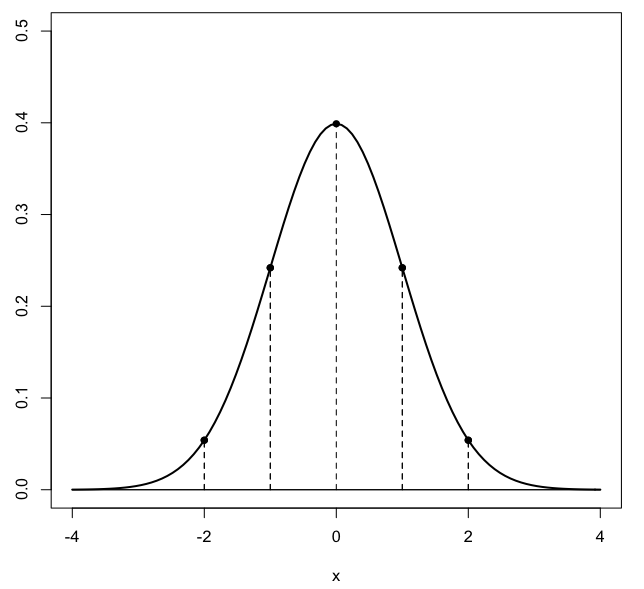
\includegraphics [scale=0.4] {gauss3.png} \end{center}
% \begin{bmatrix} a  &  b \\ c  &  d \end{bmatrix}
% \bigg |_

\Large
\noindent
This quick write-up is about the parabola.  Let's start by considering parabolas in standard orientation, i.e. that open up and have their axis of symmetry pointed straight up and down.

A parabola in this standard orientation whose vertex is located at the origin can be described by the very simple equation
\[ y = a x^2 \]
Notice that $(x=0,y=0)$ is a solution to this equation.

All parabolas contain a term with something (perhaps $1$) multiplied by $x^2$.  If the power of $x$ isn't $2$, the figure isn't a parabola.  

There are three operations that can be used to transform the basic parabola $y=x^2$ into any other parabola. 

First, we can multiply by a constant, usually designated $a$.  $a$ is called the "shape parameter".  You might think of $a$ as a kind of magnifying glass for the y-dimension.  

Second, we can translate (move) the parabola from the origin to a new position with its vertex at $P = (h,k)$.  And third, we can rotate the parabola, for example so that its axis of symmetry lies along the line $y = x$.

You've certainly seen this standard equation before
\[ y = ax^2 + bx + c \]
This is the equation for a parabola with the vertex at a point other than the origin.

For two parabolas that have the same shape but differ only by translation, the $a$ terms in these two equations are the same.  The difference---the extra terms
\[ bx + c \]
describe the movement, as we'll see below.

\subsection*{simple}

Let's start by thinking about the simplest parabola
\[ y = x^2 \]
\begin{center} 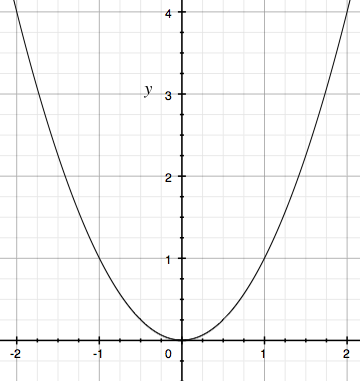
\includegraphics [scale=0.6] {para1.png} \end{center}

where, again, the standard coefficients are usually labeled as
\[ y = ax^2 + bx + c \]
In this example ($y=x^2$)
\[ a=1 \]
\[ b=0 \]
\[ c=0 \]
The parabola points up.  As $x$ gets large, $y$ gets very large.

Notice that $x^2$ is always positive or zero; hence the minimum value of $y$ is $0$, and the corresponding $x$ is also $0$, and thus the vertex, the point at which $y$ is a minimum, is at $(0,0)$.

A general way of calculating the $x$ coordinate of the vertex, when it's not at $x=0$, is to use the equation

\[ x = -\frac{b}{2a} \]
In this case 
\[ x = -\frac{0}{2} = 0 \]
The above equation can be derived from calculus but also by algebraic manipulation, as we'll see below.

Let's next consider two things we might do to this parabola to change it:  one is to modify the shape to rise either more quickly or more slowly, and the second is to change the location of the vertex.

As we said, the coefficient $a$ is called the "shape parameter".  The larger the magnitude of $a$, the steeper the curve.  (If $a$ is negative, the parabola opens downward). 

Keeping the origin at $(0,0)$, with
\[ a = 1, \ \  y = ax^2 = x^2 \]
so 
\[ x = \pm 1, y=(\pm 1)^2 = 1 \]
\[ x = \pm 2, y=(\pm 2)^2 = 4 \]
whereas if $a=2$ then
\[ y = 2x^2 \]
\[ x = \pm 1, y=2(\pm 1)^2 = 2 \]
\[ x = \pm 2, y=2(\pm 2)^2 = 8 \]

\subsection*{translation}

Suppose the vertex of the parabola $y=x^2$ is at $P=(2,1)$.  

\begin{center} 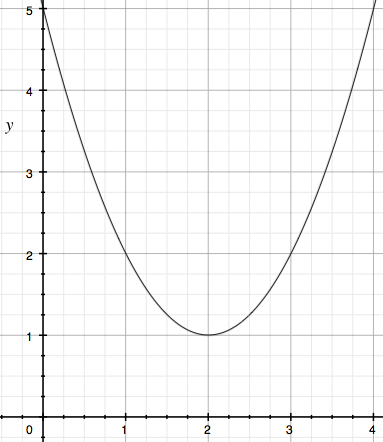
\includegraphics [scale=0.6] {para1b.png} \end{center}

The letters $h$ and $k$ are traditionally used for these values, which are constants for any particular parabola.  For example, here $h=2$ and $k=1$, given the vertex at $(2,1)$.

We write the equation of this parabola
\begin{equation}
 \boxed{(y-k) = a(x-h)^2 }
\end{equation}  

It may seem counterintuitive that the equation has minus signs (i.e. $y-k$ \emph{and} $x-h$).
\[ (y-1) = (x-2)^2 \]
Even though the equation has $(y-k)$ the y-value at the vertex is $k$.

One way to remember see is to put the $k$ on the other side
\[ y = (x-h)^2 + k \]
Now it's clear that for positive $k$, every $y$ is shifted \emph{up} by $k$ units.

If we multiply this out (using $a$ to be completely general) we obtain
\[ y = a(x-h)^2 + k \]
\[ y = ax^2 - 2axh + ah^2 + k \]

So, comparing the two forms 

\[ y = ax^2 + bx + c \]
\[ y = ax^2 - 2axh + ah^2 + k \]
We see that the coefficient of the $x$ term is $-2ah$, so that $b$ is
\[ b = -2ah \]
\begin{equation}
  \boxed{h = -\frac{b}{2a}}
\end{equation}
This is the equation we used above in finding the vertex.  If we know $a$ and $b$ we can calculate $h$, obtaining the $x$-value at the vertex.  Furthermore, from the above result
\[  c = ah^2 + k \]
\begin{equation}
\boxed{ k = c - ah^2 = c - \frac{b^2}{4a} }
\end{equation}
or alternatively, just plug $x=h=-b/2a$ into the original equation.

When we're given an equation in the form $y = ax^2 + bx + c$ and asked to find the vertex $(h,k)$, this is how it's done.

Since the shape factor $a$ is independent of $h$ and $k$, most problems with parabolas can be considered using the version with its vertex at the origin, without loss of generality.

\subsection*{roots}

The roots of the equation are the points where $y = 0$ so that
\[ y = 0 = ax^2 + bx + c \]
You can solve this either by factoring (in favorable cases) or by using the quadratic formula
\begin{equation}
\boxed {x = \frac{-b \pm \sqrt{b^2 - 4ac}}{2a} }
\end{equation}
Also, I'm sure you know that if the parabola just touches the x-axis then the discriminant $D = b^2 - 4ac = 0$, whereas if the parabola does not cross the x-axis then there are no (real) roots and $D<0$.

\subsection*{quadratic}

It's not too hard to derive the quadratic equation, so I think we should take a crack at it.  We will "complete the square."  First rearrange
\[ y = ax^2 + bx + c \]
\[ \frac{(y-c)}{a} = x^2 + \frac{bx}{a} \]
The crucial step is to observe that if we add the correct amount to the right-hand side, it can be factored

\[ x^2 + \frac{bx}{a} + (\frac{b}{2a})^2 = (x + \frac{b}{2a})(x + \frac{b}{2a}) = (x + \frac{b}{2a})^2 \]
Of course, to maintain the equality we must add the same term to the left-hand side

\[ \frac{(y-c)}{a} + (\frac{b}{2a})^2 \]
\[ \frac{1}{a} (y - c + \frac{b^2}{4a} ) \]
Combining the two results
\[ \frac{1}{a} (y - c + \frac{b^2}{4a} ) = (x + \frac{b}{2a})^2 \] 
\[ y-c + \frac{b^2}{4a} = a(x + \frac{b}{2a})^2 \]
You may recognize $h$ and $k$ in this completed square (or rather $-h$ and $-k$), but if not, take a moment to go back and compare with the equations we had before.  

Now, the roots are just the points when $y=0$ and so

\[  -c + \frac{b^2}{4a} = a(x + \frac{b}{2a})^2 \]
\[  \frac{-4ac+b^2}{4a} = a(x + \frac{b}{2a})^2 \]
\[  \frac{b^2-4ac}{4a^2} = (x + \frac{b}{2a})^2 \]
\[  \pm \frac{\sqrt{b^2-4ac}}{2a} = x + \frac{b}{2a} \]
\[  x = \frac{-b \pm \sqrt{b^2-4ac}}{2a} \]
which is the quadratic equation.

\subsection*{focus and directrix}

\begin{center} 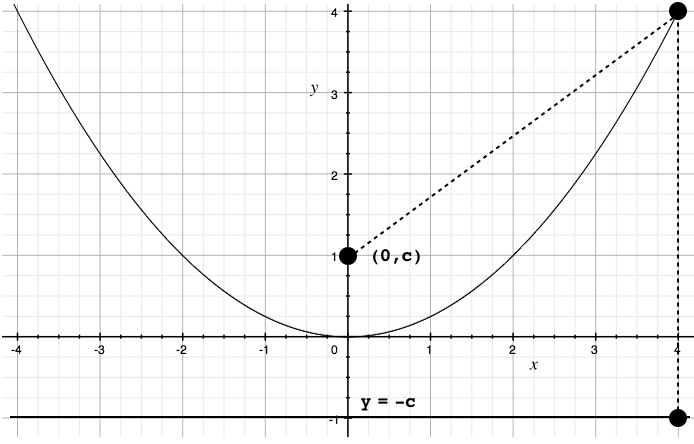
\includegraphics [scale=0.5] {para3.png} \end{center}

A classical result about parabolas concerns the focus and the directrix.  The directrix is defined as a horizontal line passing below the parabola, and the focus as a point on the axis of symmetry above the vertex.

These are positioned so that the distance $c$ from the vertex to the focus is the same as the distance from the vertex vertically down to the directrix.  (This $c$ is \emph{not} the same as the one in the standard formula for a parabola).

We haven't said yet what the value of $c$ is. The claim is that for the correct value of $c$, the distance from any point on the parabola to the focus will be equal to the distance vertically down to the directrix.

The parabola shown has the equation $y=\frac{1}{4}x^2$.  That is, $a = \frac{1}{4}$.  For this parabola, $c=1$.

To derive this result, consider a general point on the parabola, $Q=(x, ax^2)$.  The vertical distance down to the directrix is just 

\[ d_d = ax^2 + c \]

We'll square this for use below

\[ {d_d}^2 = (ax^2 + c)^2 \]

The other is given by the Pythagorean Theorem

\[ {d_f}^2 = x^2 + (ax^2 - c)^2 \]

Our claim is that these two distances should be equal, so the squares should also be equal

\[ (ax^2 + c)^2 = x^2 + (ax^2 - c)^2 \]
\[ a^2x^4 + 2ax^2c + c^2 = x^2 + a^2x^4 - 2ax^2c + c^2 \]
\[ 2ax^2c = x^2 - 2ax^2c \]
\[ 4ax^2c = x^2 \]
\begin{equation}
\boxed {4ac = 1}
\end{equation}

For example, if $a = 1$, $c = \frac{1}{4}$.

Probably the most interesting property of the parabola is that any light ray coming down vertically will bounce off the surface of the parabola so that it is reflected to the focus.  Reflecting telescopes are made in this way.  The reverse is also true.  The inside of a headlight has a parabolic shape, so that the light coming out is focused into a parallel beam.

\subsection*{rotation}

The last thing that can happen to make life complicated is a rotation of the parabola.  You are probably used to seeing examples where it opens to the right or left.  These are obtained by having an equation like
\[ a(y-k)^2 = (x-h)  \]
with $x = g(y)$
Then, the easiest thing to do is to switch $x$ for $y$, solve the problem, and switch back at the end.

But it is also possible to rotate through a different angle, like $45^\circ$.  What happens then?  Well, basically we replace $x$ and $y$ by $u$ and $v$ with
\[ x = u \ cos \ \theta - v \ sin \ \theta \]
\[ y = u \ sin \ \theta + v \ cos \ \theta \]
(I derived these in a separate write-up).
For $45^\circ$, $sin \ \theta = cos \ \theta = 1/ \sqrt{2}$.
Let
\[ k = sin \ \theta = cos \ \theta = 1/ \sqrt{2} \]
Substitute for $x$ and $y$ as given above
\[ y = ax^2 + bx + c \]
\[ ku + kv = a(ku - kv)^2 + b(ku - kv) + c \]
\[ u + v = ak(u^2 - 2uv + v^2) + b(u - v) + \frac{c}{k} \]

Now, we might attempt to solve this for $v$ in terms of $u$, but there is a new term $-2uv$ which mixes up $u$ and $v$.  That is what gives a parabola that is not symmetric with respect to either the x-axis or the y-axis.

\subsection*{slope}

Using calculus, for a parabola in standard orientation, we can find the slope of the tangent line to the curve at any point by taking the derivative

\[ m = \frac{d}{dx} (ax^2 + bx + c) = 2ax + b \]

The slope of the tangent is zero at the vertex

\[ m = 2ax + b = 0 \]
\[ x = -\frac{b}{2a} \]
as we saw before.

\subsection*{parallel rays are reflected to the focus}
Above we said that if the light source is placed at the focus of a paraboloid headlight, then rays reflected off the surface emerge "straight out" (or up, as we usually draw parabolas).  Conversely, light rays parallel to the axis of symmetry that enter a paraboloid converge at the focus.

Here is a proof of this that uses vectors.  It is not as clean as I'd like (there is a bit of algebra) but it isn't too bad.  Start with a standard parabola centered with its vertex at the origin with equation $y=ax^2$.  At any point on the parabola $P = (x,ax^2)$, the tangent line to the parabola has slope $2ax$, by the most basic result in calculus.

Draw a vector $\mathbf{u}$ from the focus $F = (0,c)$ to the point $P$.  This vector has components

\[ \mathbf{u} = \langle x, ax^2 - c \rangle \]
Draw a vector $\mathbf{v}$ extending vertically up from point $P$, its components are
\[ \mathbf{v} = \langle 0, k \rangle \]
where $k$ can be any constant.
Finally, draw the vector $\mathbf{w}$ parallel to the tangent line.  $\mathbf{w}$ has the same slope as the tangent line, so one version of it could be
\[ \mathbf{w} = \langle 1, 2ax \rangle \]

The statements above about the paths of light rays can be restated as follows:  the angle $\theta$ between $\mathbf{u}$ and $\mathbf{w}$ is equal to the angle $\phi$ between $\mathbf{v}$ and $\mathbf{w}$.  We can calculate these angles using the dot product.  Recall that

\[ \mathbf{u} \cdot \mathbf{w} = u w \cos \theta \]
\[ \mathbf{v} \cdot \mathbf{w} = v w \cos \phi \]

So if $\theta = \phi$, then $\cos \theta = \cos \phi$ and $w \cos \theta = w \cos \phi$ so that
\[ \frac{\mathbf{u} \cdot \mathbf{w}}{u} = \frac{\mathbf{v} \cdot \mathbf{w}}{v} \]
Conversely, if this equality holds, then $\theta = \phi$.

We calculate these values in the usual way:
\[ \mathbf{u} \cdot \mathbf{w} = x + 2ax (ax^2 - c) \]
\[ \mathbf{v} \cdot \mathbf{w} = 2ax k \]
\[ u = | \mathbf{u} | = \sqrt{x^2 + (ax^2 - c)^2} \]
\[ v = | \mathbf{v} | = k \]

Our equation is:
\[ \frac{\mathbf{u} \cdot \mathbf{w}}{u} = \frac{\mathbf{v} \cdot \mathbf{w}}{v} \]
From what we had above, the right-hand side is easy:
\[ \frac{\mathbf{v} \cdot \mathbf{w}}{v} = \frac{2axk}{k} = 2ax \]
We are reassured to see the arbitrary constant $k$ go away.  The left-hand side is a bit of a mess:
\[ \frac{\mathbf{u} \cdot \mathbf{w}}{u}  = \frac{x + 2ax (ax^2 - c)}{\sqrt{x^2 + (ax^2 - c)^2} } \]

So what we need to do is prove that
\[ \frac{x + 2ax (ax^2 - c)}{\sqrt{x^2 + (ax^2 - c)^2} } = 2ax \]
\[ x + 2ax (ax^2 - c) = 2ax \sqrt{x^2 + (ax^2 - c)^2} \]
We can factor out one $x$ right away
\[ 1 + 2a (ax^2 - c) = 2a \sqrt{x^2 + (ax^2 - c)^2} \]
Expand a little bit
\[ 1 + 2a^2x^2 - 2ac = 2a \sqrt{x^2 + (ax^2 - c)^2} \]

And now we just have to do the grunt work of squaring both sides.  The left-hand side is
\[ (1 + 2a^2x^2 - 2ac)^2 \]
\[ = 1 + 2a^2x^2 - 2ac + 2a^2x^2 + 4a^4x^4 - 4a^3cx^2 - 2ac - 4a^3cx^2 + 4a^2c^2 \]
\[ = 1 + 4a^2x^2 - 4ac + 4a^4x^4 - 8a^3cx^2 + 4a^2c^2 \]
while the square of the right-hand side is
\[ 4a^2 \ [ \ x^2 + (ax^2 - c)^2 \ ] \]
\[ = 4a^2(x^2 + a^2x^4 - 2acx^2 + c^2) \]
\[ = 4a^2x^2 + 4a^4x^4 - 8a^3cx^2 + 4 a^2c^2 \]

We see that each term on the right-hand side has a matching term on the left-hand side.  All of these can be canceled, leaving 
\[ 1 - 4ac = 0 \]

But recall from the section on \textbf{focus and directrix} that $4ac = 1$.  Thus, all the terms cancel, and we have shown that the two sides are equal.  So indeed
\[ \frac{\mathbf{u} \cdot \mathbf{w}}{u} = \frac{\mathbf{v} \cdot \mathbf{w}}{v} \]
and therefore
\[ w \cos \theta = w \cos \phi \]
and so
\[ \theta = \phi \]
\subsection*{alternate proof}
\begin{center} 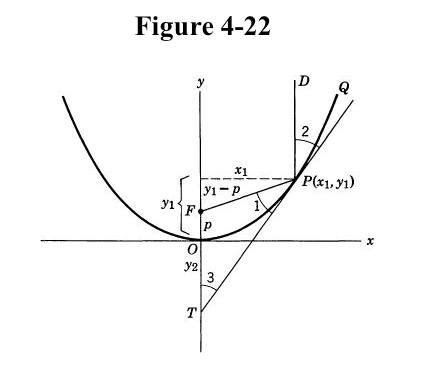
\includegraphics [scale=0.6] {Kline_4_22.png} \end{center}
Morris Kline has an alternate proof in his book \emph{Calculus}.  In the figure we need to show that angles $1$ and $2$ are equal.  By standard geometry angles $2$ and $3$ are equal, hence we need to show that angles $1$ and $3$ are equal.  We do this by showing that $FP$ is equal to $FT$.

Rather than substitute for $y = ax^2$ we just leave things in terms of $y$.  Notice that the diagram uses $p$ for the distance from the origin to the focus, and labels $P = (x_1,y_1)$.  Using Pythagoras, as indicated, the distance $FP$ is 
\[ FP = \sqrt{x_1^2 + (y_1-p)^2} \]

To get $FT$ we need to find what is labeled as $y_2$, the intercept of the tangent line with the $y$-axis.  We get this from the point-slope formula:
\[ \frac{y_1 + y_2}{x_1} = 2ax_1 \]
\[ y_1 + y_2 = 2ax_1^2 \]
But of course $y_1 = ax_1^2$ and so
\[ y_1 + y_2 = 2y_1 \]
Thus $y_1 = y_2$ and hence $FT = y_1 + p$.

Going back to $FP$, we use the same crucial fact about the focus that we relied on in the first proof, namely that $4ap = 1$ and so
\[ y_1 = ax_1^2 \]
\[ x_1^2 = 4p y_1 \]
Our previous expression was
\[ FP = \sqrt{x_1^2 + (y_1-p)^2} \]
substituting for $x_1^2$
\[ FP = \sqrt{4py_1 + (y_1-p)^2} \]
\[ = \sqrt{4py_1 + y_1^2 - 2y_1p +  p^2} \]
\[ = \sqrt{y_1^2 + 2y_1p +  p^2} \]
\[ = \sqrt{(y_1 + p)^2} \]
\[ FP = y_1 + p \]
$FT$ and $FP$ are the same length, and so the two angles are equal.  Also, we showed that $FP = y + p$, which means that every point on the parabola has the distance $y + p$ to the focus, as well as the vertical distance $y + p$ to a horizontal line a distance of $p$ below the $x$-axis and parallel to it.  This line is the directrix.

\end{document}  